\appendix

\begin{table}[h]
  \centering
  \begin{tabular}{S  S S S S}
    \toprule
    {$\nu\:/\:\si{\kilo\hertz}$}& {$U_1\:/\:\si{\milli\volt}$}& {$U_\text{A}\:/\:\si{\milli\volt}$}&{$V'$}& {$\phi\:/\:\si{\degree}$}\\
    \midrule
    1.1 & 570 & 570 & 1.0 & 180\\
    1.5 & 540 & 540 & 1.0 & 180\\
    15.1 & 540 & 540 & 1.0 & -174\\
    150.0 & 540 & 570 & 1.1 & -161\\
    209.0 & 590 & 610 & 1.0 & -2\\
    275.0 & 590 & 500 & 0.8 & -130\\
    453.0 & 600 & 330 & 0.6 & -101\\
    981.0 & 590 & 170 & 0.3 & -70\\
    1500.0 & 590 & 120 & 0.2 & -24\\
    \bottomrule
  \end{tabular}
  \caption{Werte der Widerstandskombination $R_1 = \SI{9.96(5)}{\kilo\ohm}$, $R_\text{N} = \SI{9.96(5)}{\kilo\ohm}$; im Folgenden als 1. Widerstandskombination bezeichnet.}
  \label{tab:gegen_kombi_1}
\end{table}
\begin{table}[h]
  \centering
  \begin{tabular}{S  S S S S}
    \toprule
    {$\nu\:/\:\si{\kilo\hertz}$}& {$U_1\:/\:\si{\milli\volt}$}& {$U_\text{A}\:/\:\si{\milli\volt}$}&{$V'$}& {$\phi\:/\:\si{\degree}$}\\
    \midrule
    1.0 & 615 & 64 & 0.1 & -174\\
    1.5 & 615 & 64 & 0.1 & -174\\
    15.0 & 620 & 64 & 0.1 & -172\\
    150.0 & 590 & 69 & 0.12 & -163\\
    209.0 & 580 & 70 & 0.12 & -160\\
    275.0 & 580 & 75 & 0.13 & -158\\
    600.0 & 580 & 105 & 0.18 & -122\\
    800.0 & 580 & 110 & 0.19 & -86\\
    1100.0 & 580 & 110 & 0.19 & -49\\
    1850.0 & 590 & 84 & 0.14 & 0\\
    \bottomrule
  \end{tabular}
  \caption{Werte der Widerstandskombination $R_1 = \SI{9.96(5)}{\kilo\ohm}$, $R_\text{N} = \SI{1.002(50)}{\kilo\ohm}$; im Folgenden als 2. Widerstandskombination bezeichnet.}
  \label{tab:gegen_kombi_2}
\end{table}

\begin{table}[h]
  \centering
  \begin{tabular}{S S S S S}
    \toprule
    {$\nu\:/\:\si{\kilo\hertz}$}& {$U_1\:/\:\si{\milli\volt}$}& {$U_\text{A}\:/\:\si{\milli\volt}$}&{$V'$}& {$\phi\:/\:\si{\degree}$}\\
    \midrule
    1.0 & 580 & 1150 & 2.0 & 185\\
1.5 & 580 & 1150 & 2.0 & 185\\
15.0 & 580 & 1150 & 2.0 & -172\\
30.0 & 580 & 1180 & 2.0 & -165\\
50.0 & 580 & 1160 & 2.0 & -162\\
75.0 & 570 & 1150 & 2.0 & -158\\
120.0 & 580 & 1090 & 1.9 & -144\\
200.0 & 590 & 840 & 1.4 & -119\\
500.0 & 600 & 390 & 0.6 & -80\\
1000.0 & 590 & 260 & 0.4 & -68\\
2000.0 & 600 & 295 & 0.5 & -29\\
    \bottomrule
  \end{tabular}
  \caption{Werte der Widerstandskombination $R_1 = \SI{1.002(50)}{\kilo\ohm}$, $R_\text{N} = \SI{470(5)}{\ohm}$; im Folgenden als 3. Widerstandskombination bezeichnet.}
  \label{tab:gegen_kombi_3}
\end{table}
\begin{table}[h]
  \centering
  \begin{tabular}{S  S S S S}
    \toprule
    {$\nu\:/\:\si{\kilo\hertz}$}& {$U_1\:/\:\si{\milli\volt}$}& {$U_\text{A}\:/\:\si{\milli\volt}$}&{$V'$}& {$\phi\:/\:\si{\degree}$}\\
    \midrule
    1.0 & 890 & 8400 & 9.4 & -173\\
1.5 & 880 & 8400 & 9.5 & -173\\
5.0 & 890 & 8800 & 9.9 & -170\\
15.0 & 930 & 9000 & 9.7 & -158\\
50.0 & 900 & 3900 & 4.3 & -108\\
100.0 & 900 & 1870 & 2.1 & -95\\
250.0 & 900 & 780 & 0.9 & -82\\
750.0 & 930 & 300 & 0.3 & -55\\
1000.0 & 930 & 220 & 0.2 & -50\\
2500.0 & 760 & 100 & 0.1 & -30\\
3100.0 & 790 & 100 & 0.1 & -2\\
    \bottomrule
  \end{tabular}
  \caption{Werte der Widerstandskombination $R_1 = \SI{9.96(5)}{\kilo\ohm}$, $R_\text{N} = \SI{1.002(50)}{\kilo\ohm}$; im Folgenden als 4. Widerstandskombination bezeichnet.}
  \label{tab:gegen_kombi_4}
\end{table}

\begin{table}[h]
  \centering
  \begin{tabular}{S  S S S}
    \toprule
    {$\omega\:/\:\si{\hertz}$}& {$U_\text{A}\:/\:\si{\milli\volt}$}& {$U_1\:/\:\si{\milli\volt}$}&{$V'$}\\
    \midrule
    31.42 & 318.0 & 590 & 0.54\\
    62.83 & 101.0 & 590 & 0.17\\
    94.25 & 115.0 & 590 & 0.19\\
    125.66 & 80.0 & 600 & 0.13\\
    157.08 & 72.0 & 570 & 0.13\\
    188.5 & 41.0 & 590 & 0.07\\
    314.16 & 28.1 & 590 & 0.05\\
    471.24 & 22.5 & 590 & 0.04\\
    628.32 & 20.9 & 590 & 0.04\\
    942.48 & 16.1 & 590 & 0.03\\
    \bottomrule
  \end{tabular}
  \caption{Werte des Umkehr-Integrators mit den Fehlern $\sigma_\nu = \SI{5}{\hertz}$ und $\sigma_U = \SI{5}{\milli\volt}$.}
  \label{tab:int_werte}
\end{table}

\begin{table}[h]
  \centering
  \begin{tabular}{S  S S S}
    \toprule
    {$\omega\:/\:\si{\hertz}$}& {$U_\text{A}\:/\:\si{\milli\volt}$}& {$U_1\:/\:\si{\milli\volt}$}&{$V'$}\\
    \midrule
    62.83 & 60.0 & 600 & 0.1\\
    157.08 & 115.0 & 600 & 0.19\\
    314.16 & 205.0 & 600 & 0.34\\
    628.32 & 390.0 & 600 & 0.65\\
    942.48 & 550.0 & 590 & 0.93\\
    1256.64 & 750.0 & 600 & 1.25\\
    1884.96 & 1130.0 & 600 & 1.88\\
    3141.59 & 1770.0 & 590 & 3.0\\
    4398.23 & 2570.0 & 600 & 4.28\\
    6283.19 & 3540.0 & 590 & 6.0\\
    \bottomrule
  \end{tabular}
  \caption{Werte des Umkehr-Differentiators mit den Fehlern $\sigma_\nu = \SI{5}{\hertz}$ und $\sigma_U = \SI{5}{\milli\volt}$.}
  \label{tab:diff_werte}
\end{table}

\begin{figure}
  \centering
  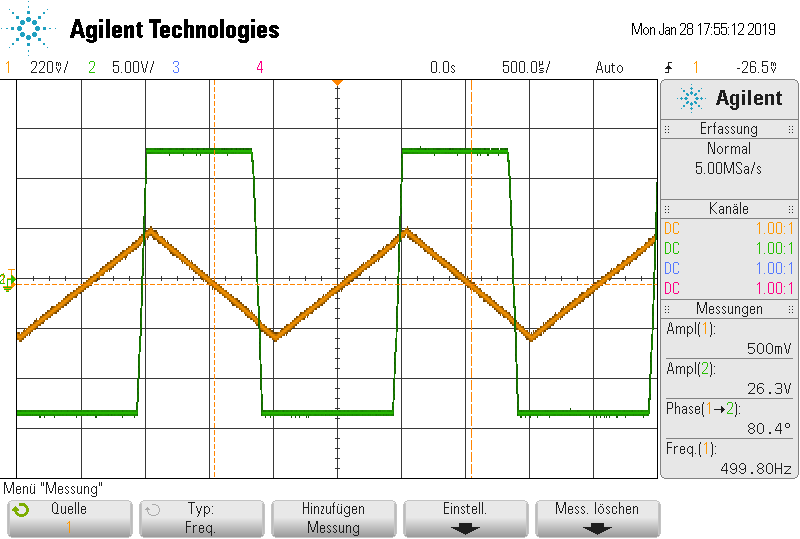
\includegraphics[width=0.8\textwidth]{Schlager/scope_23.png}
  \caption{Das Oszilloskopbild des Schmitt-Triggers mit Werten für die Amplitude. Hier ist die Eingangsspannung in orange und die Ausgangsspannung in grün zu sehen.}
  \label{fig:schmitt2}
\end{figure}
\section{Kopie der Originaldaten}
\begin{figure}
  \centering
  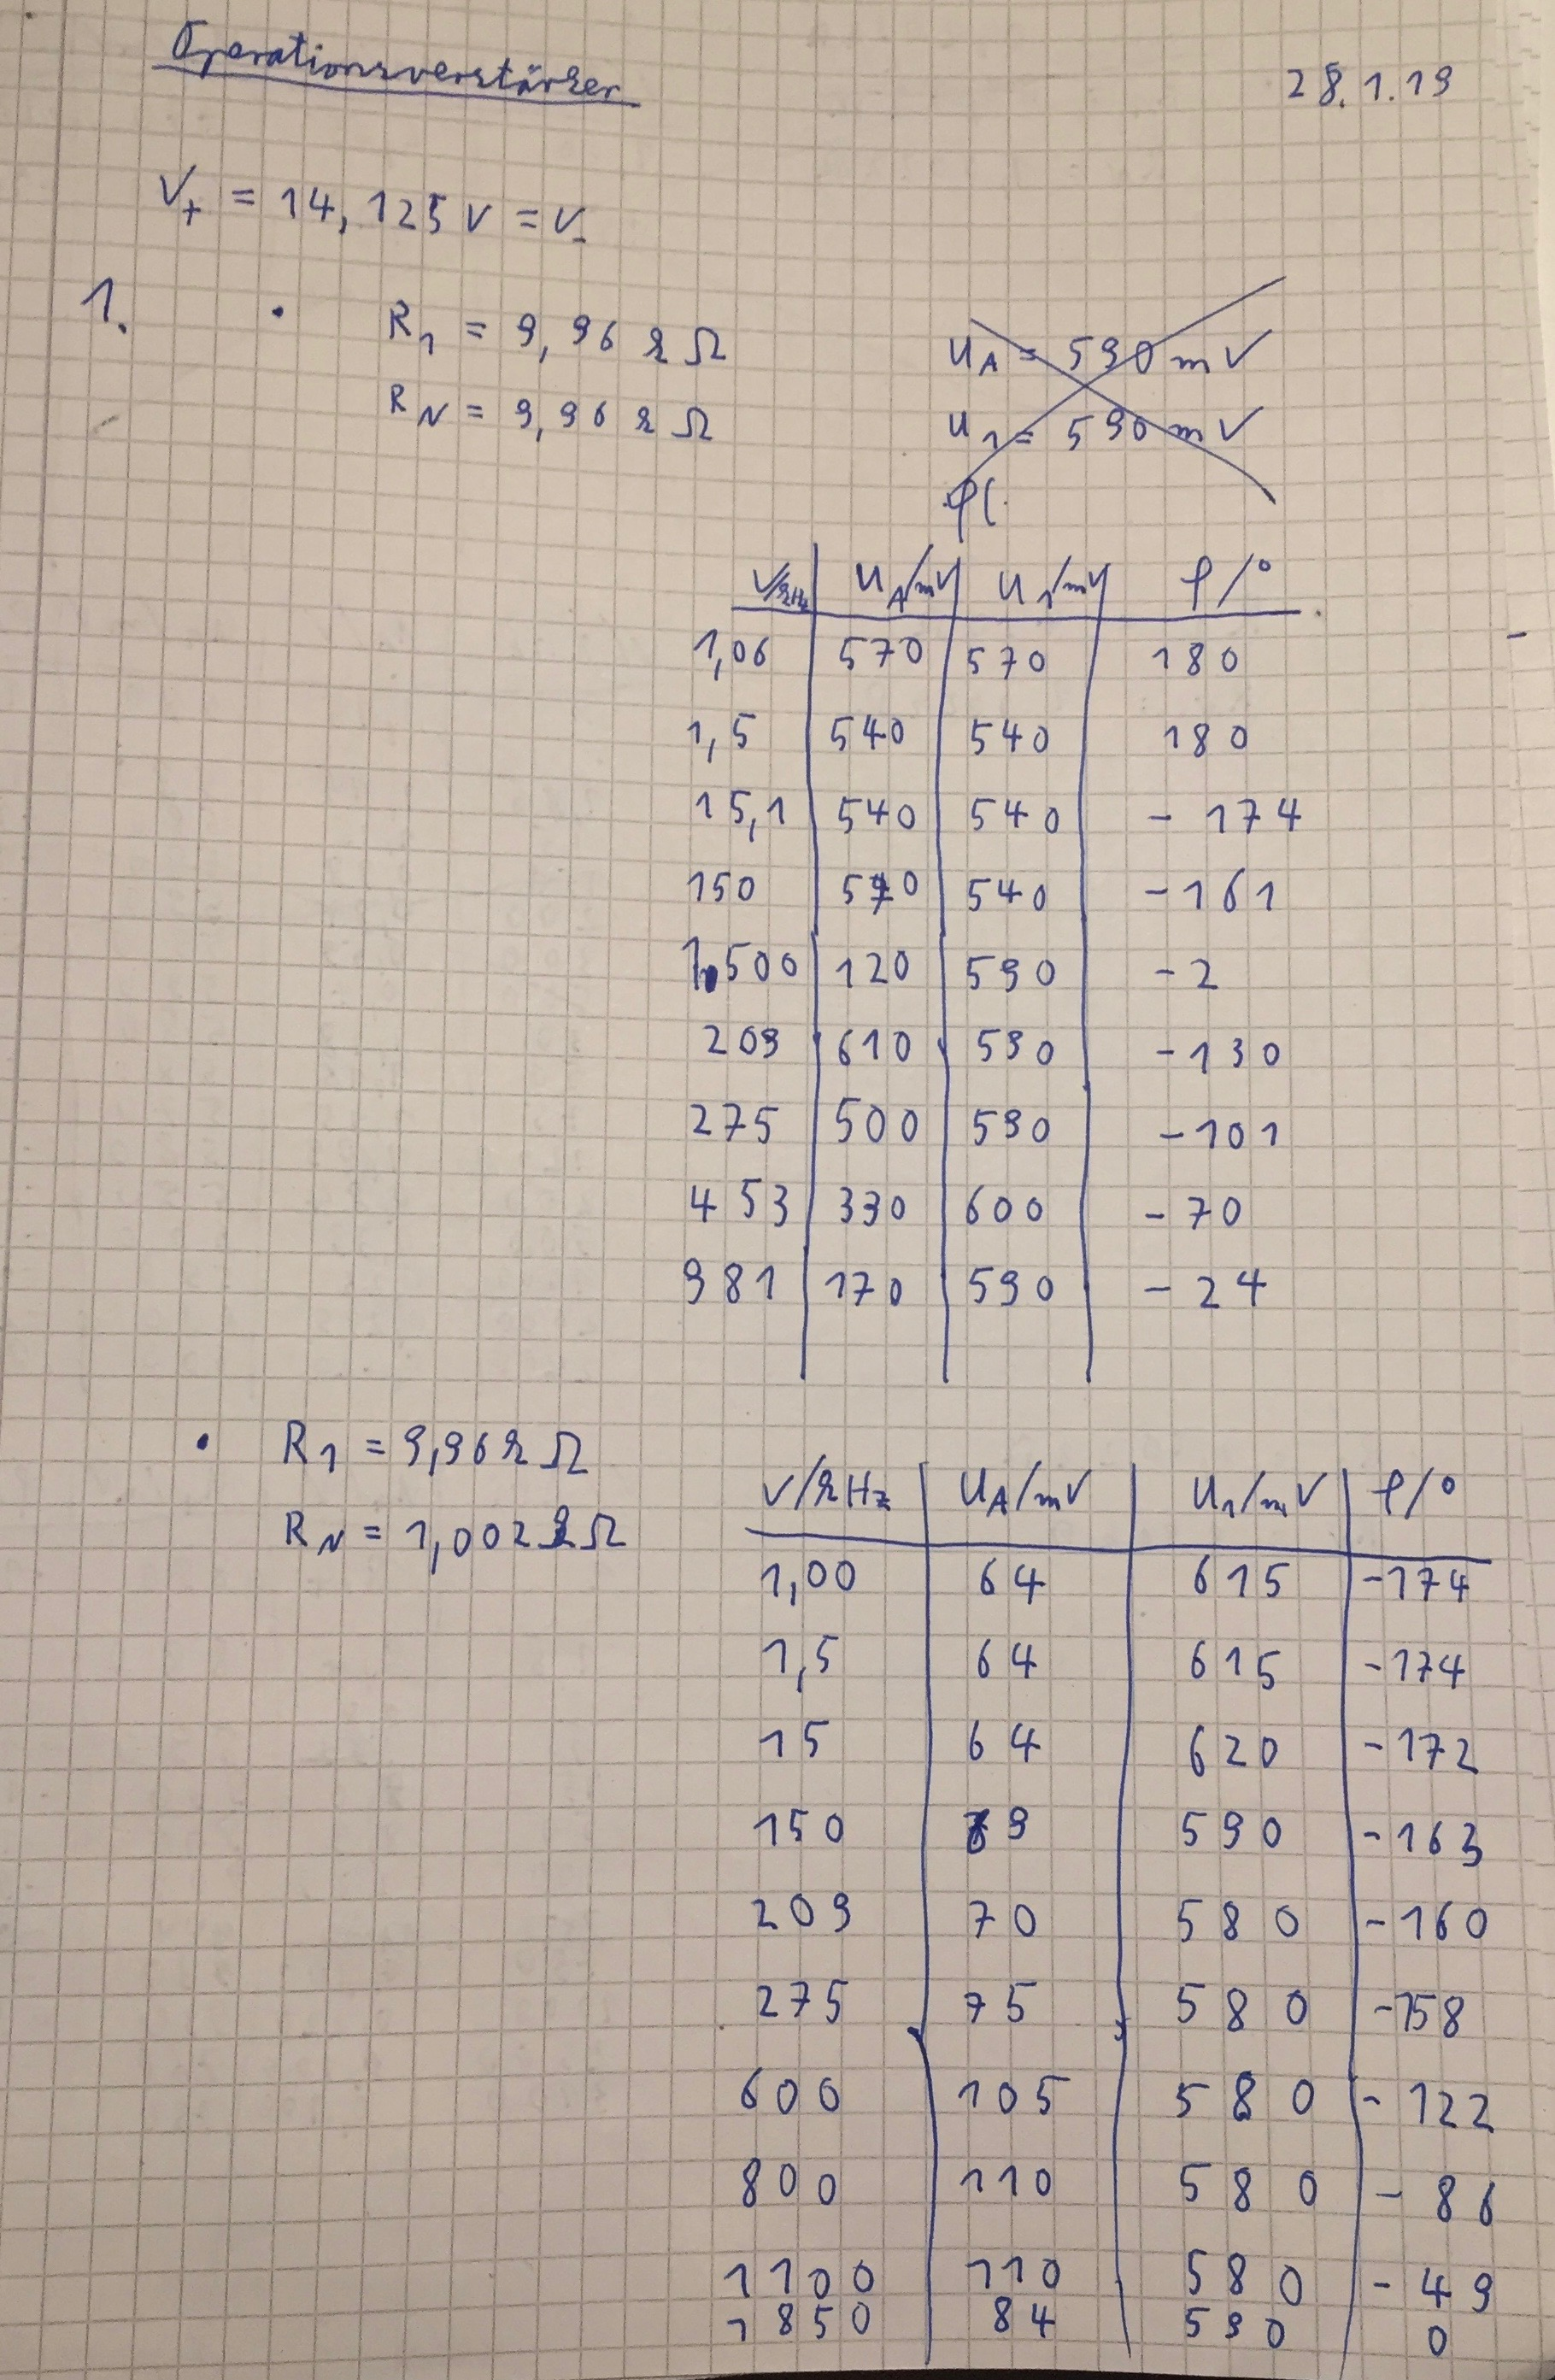
\includegraphics[width=0.8\textwidth]{Messwerte/1.jpg}
  \caption{Messwerte Teil 1.}
  \label{fig:messwerte1}
\end{figure}
\begin{figure}
  \centering
  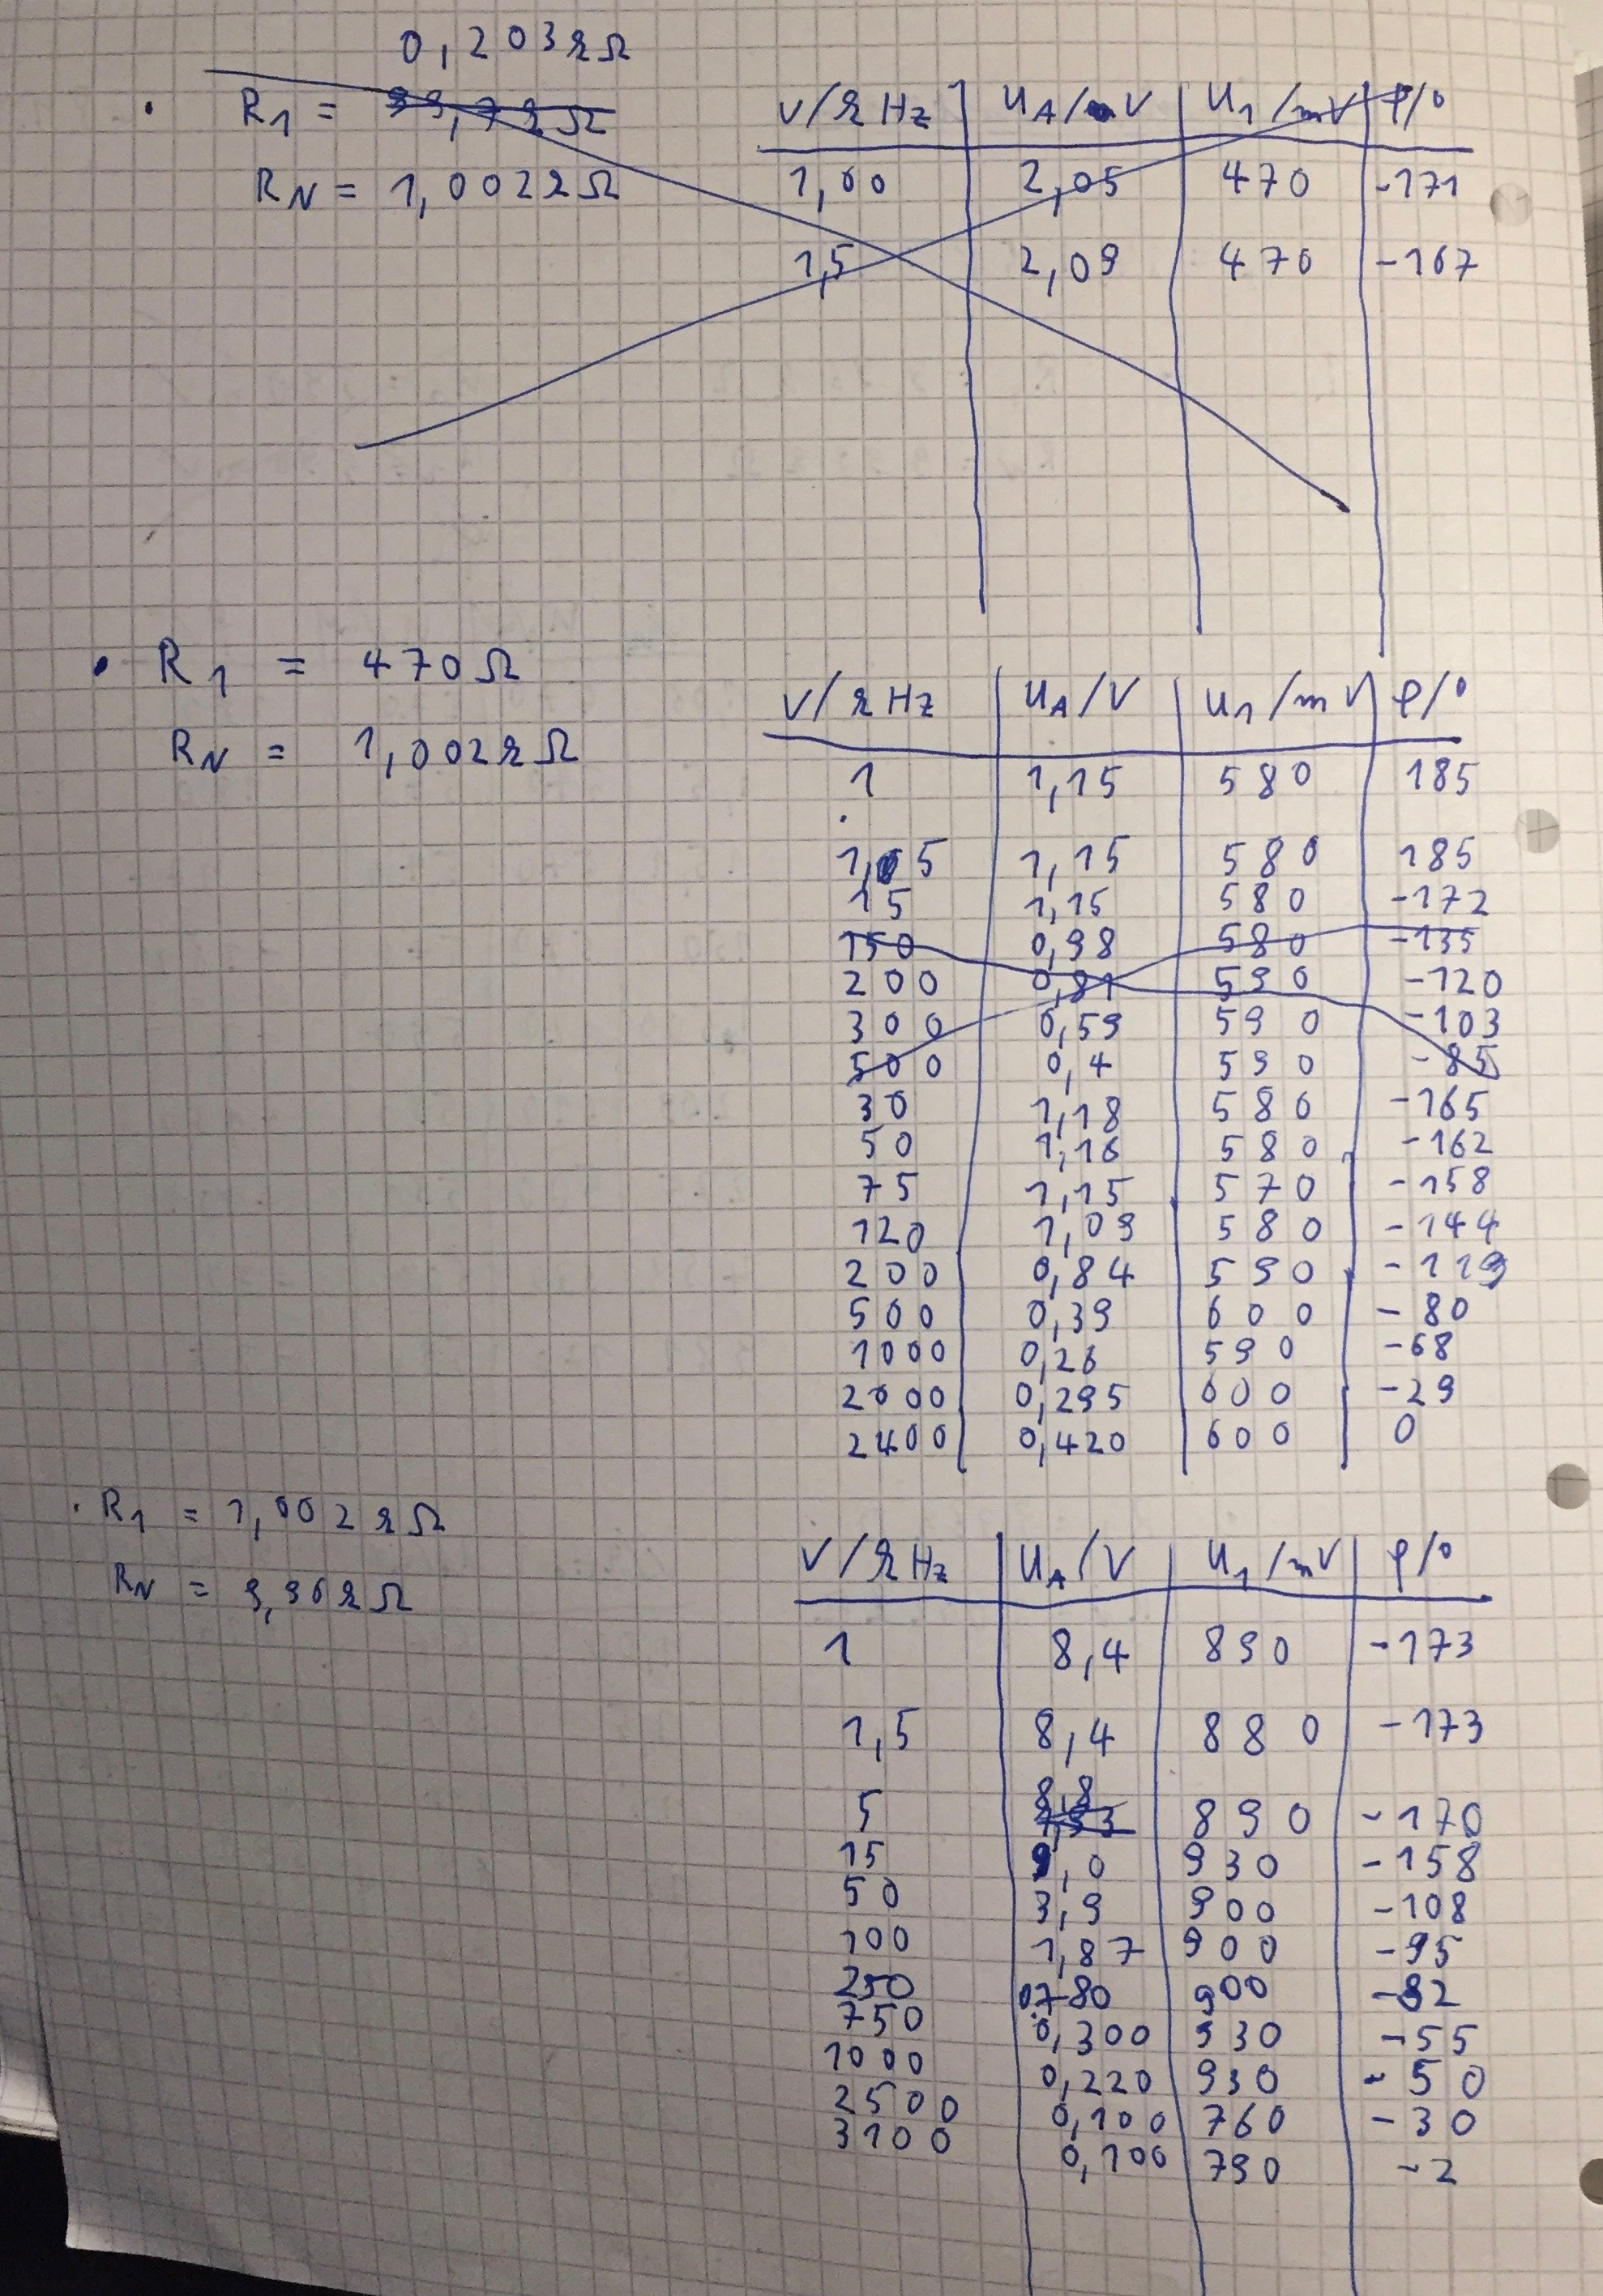
\includegraphics[width=0.8\textwidth]{Messwerte/2.jpg}
  \caption{Messwerte Teil 2.}
  \label{fig:messwerte2}
\end{figure}
\begin{figure}
  \centering
  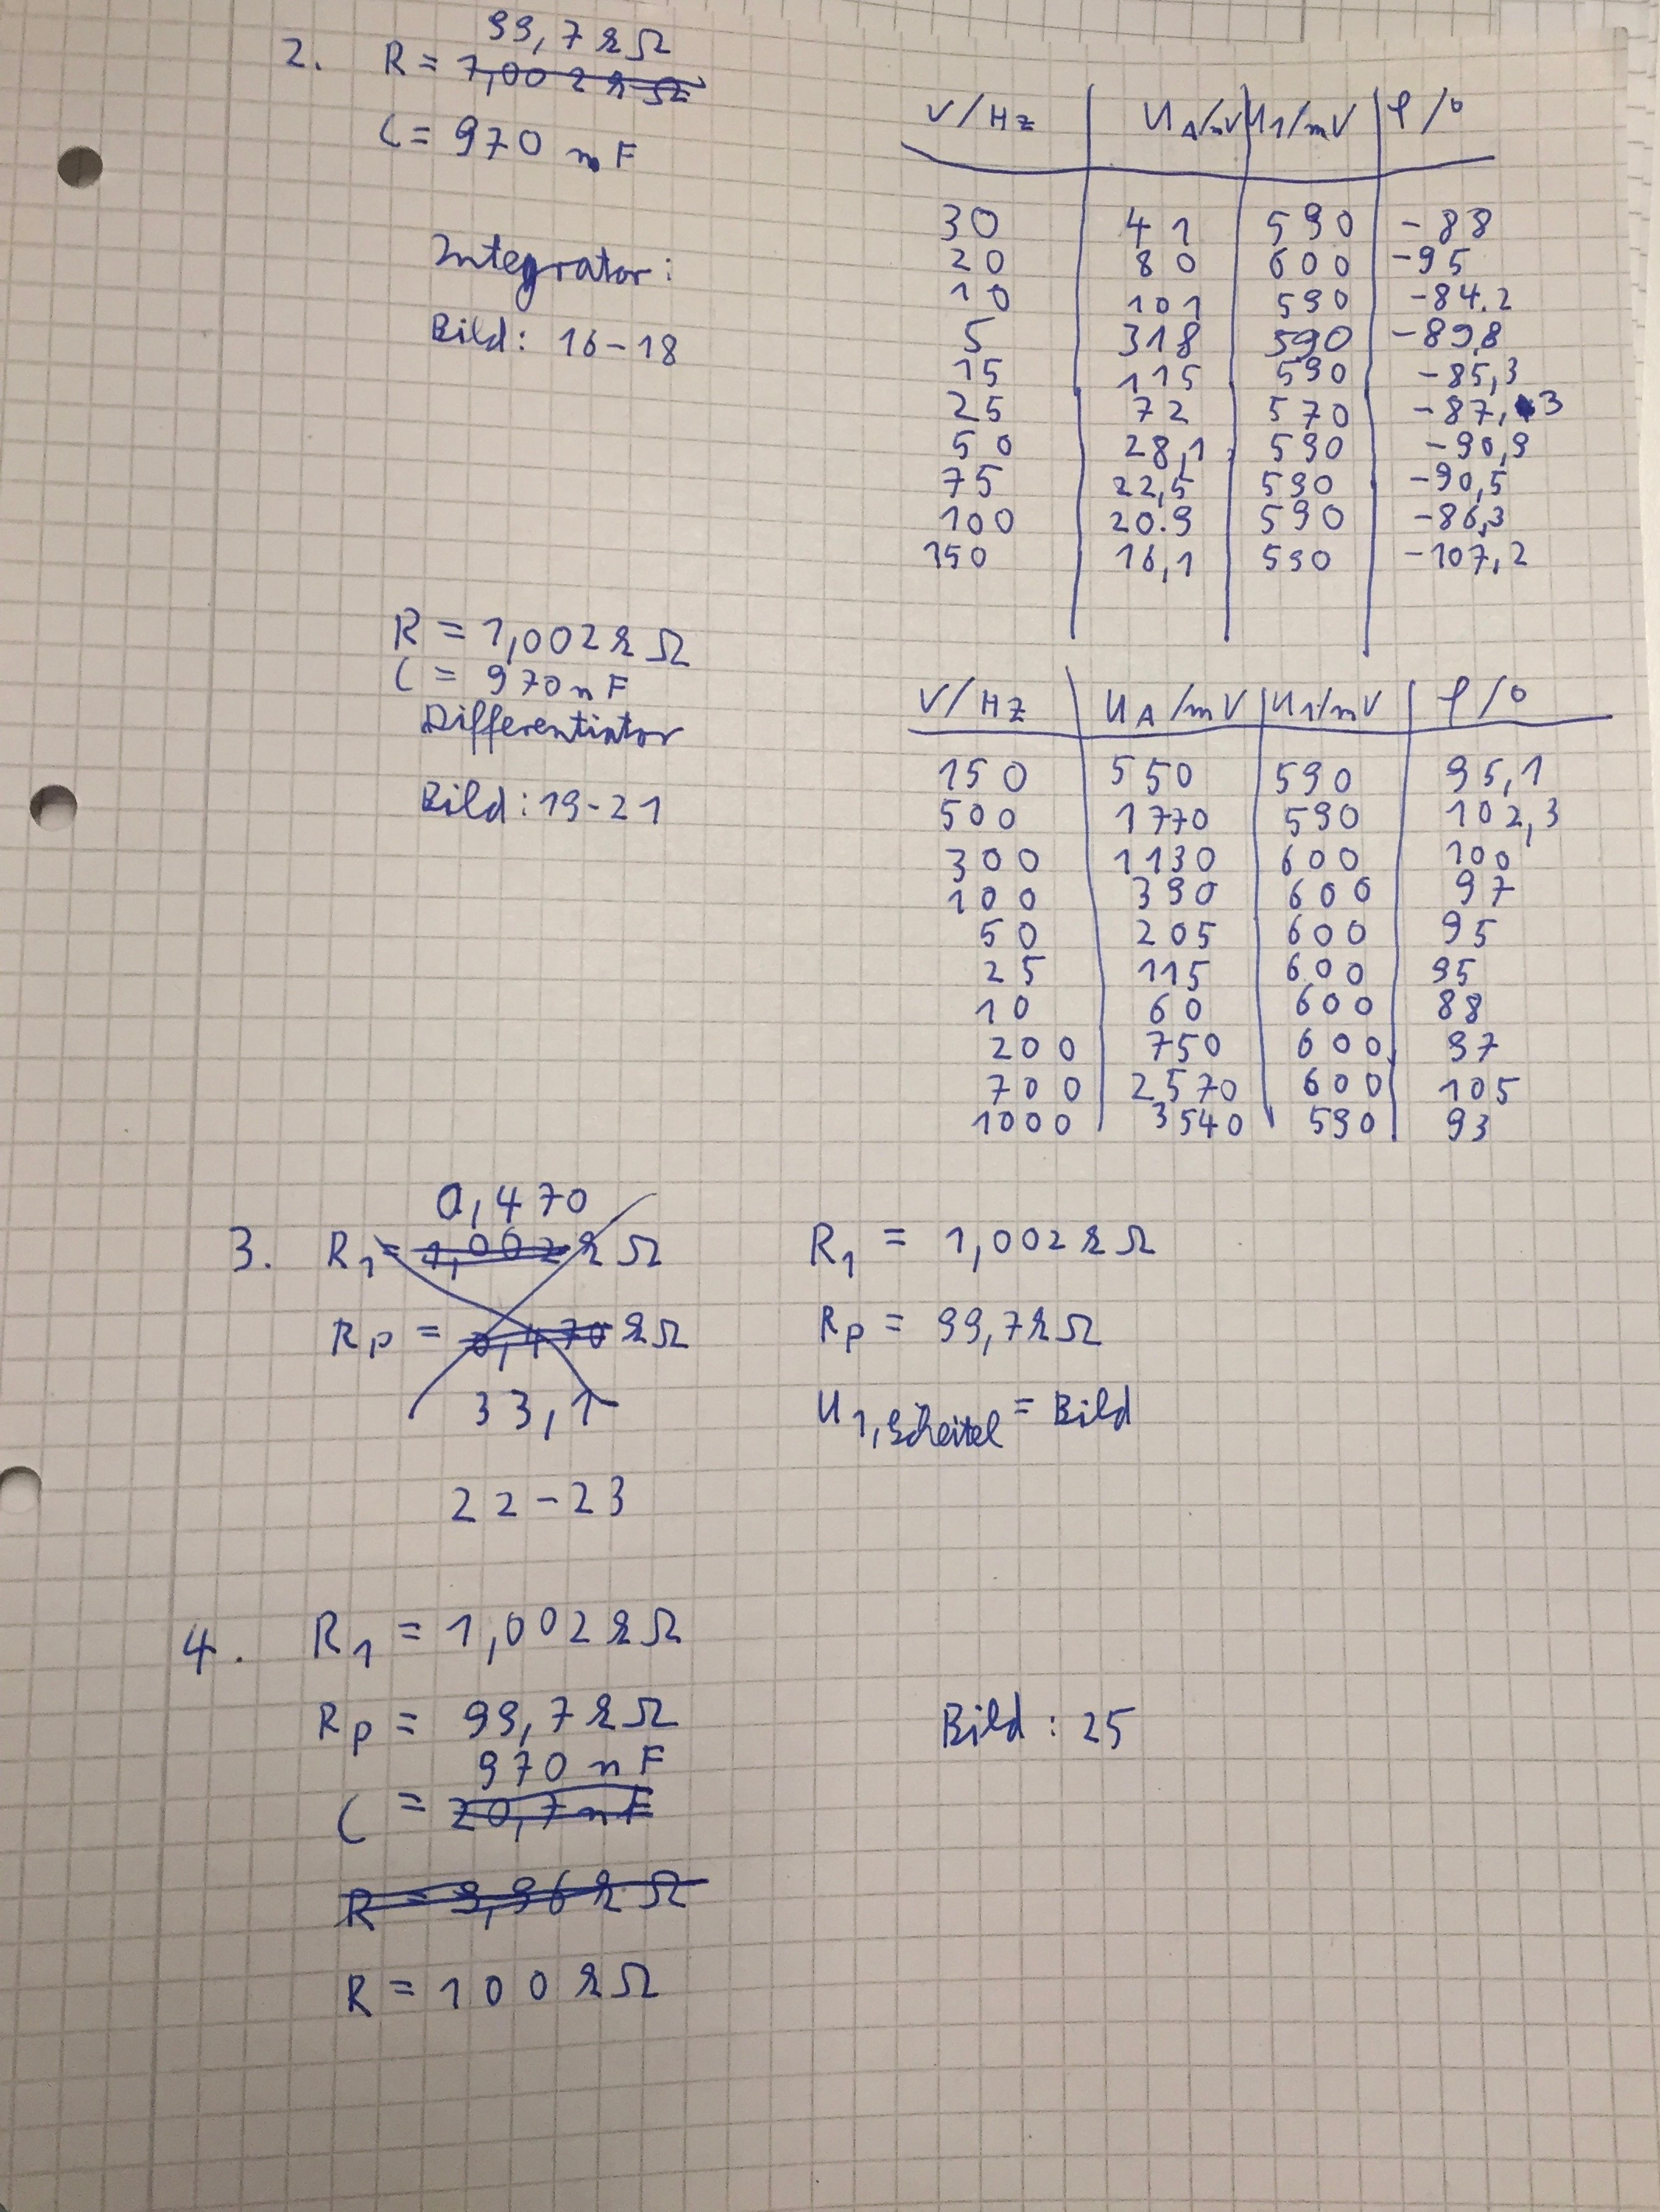
\includegraphics[width=0.8\textwidth]{Messwerte/3.jpg}
  \caption{Messwerte Teil 3.}
  \label{fig:messwerte3}
\end{figure}
\begin{figure}
  \centering
  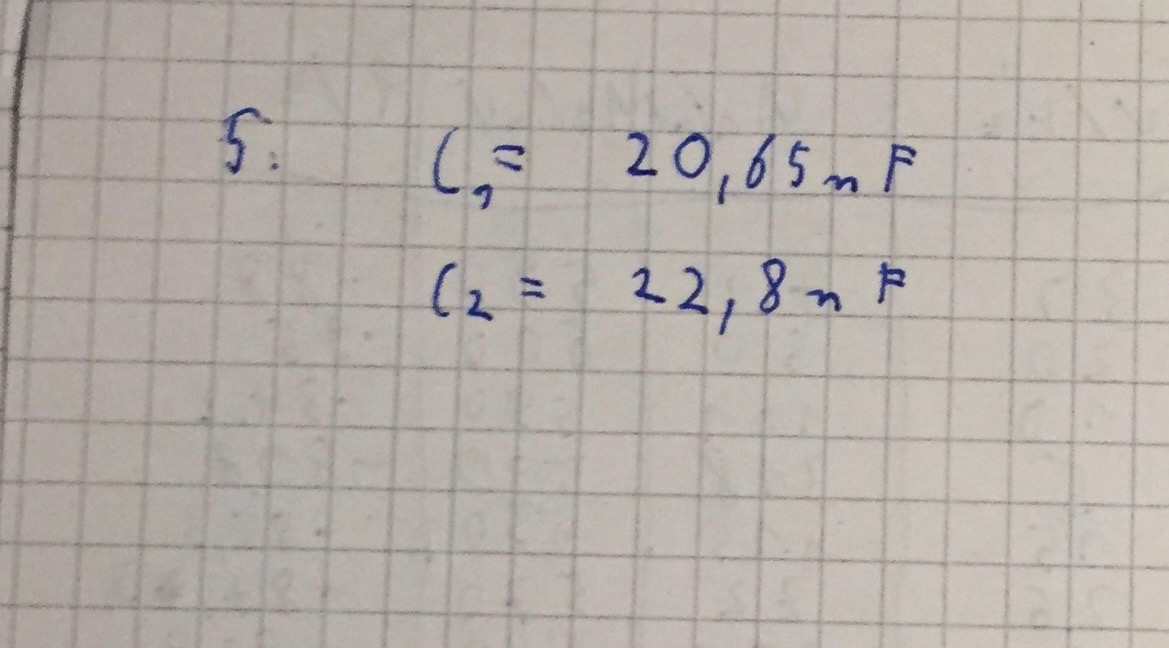
\includegraphics[width=0.8\textwidth]{Messwerte/4.jpg}
  \caption{Messwerte Teil 4.}
  \label{fig:messwerte4}
\end{figure}
